\documentclass[a4paper]{article}
\usepackage{graphicx}
\usepackage{tikz}
\usepackage{xcolor}
\graphicspath{{./subfigs}}
\usepackage[export]{adjustbox}

\pagenumbering{gobble}
\newlength{\mywidth}
\newlength{\myheight}

\usepackage[framemethod=tikz]{mdframed}
\mdfdefinestyle{mdstyle}{align=center,innertopmargin=2pt,
    innerleftmargin=1pt,innerrightmargin=0pt,innerbottommargin=2pt,backgroundcolor=gray!50,linecolor=gray!50, roundcorner=3pt}
\definecolor{gray}{RGB}{220,220,220}
\newcommand{\st}{\sffamily}
\begin{document}
\nopagecolor
\setlength{\tabcolsep}{-1pt}

\begin{mdframed}[style=mdstyle]
\resizebox{\textwidth}{!}{
\begin{tabular}{c@{\hskip 0pt} c}
    \rotatebox[origin=c]{90}{\st Sagittal}&\begin{tabular}{c}
      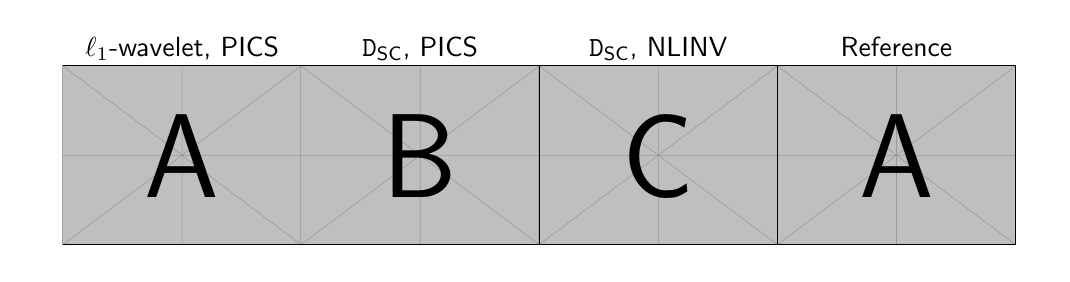
\begin{tikzpicture}
    \node[] (fig) at (0,0){
    \renewcommand{\arraystretch}{0}
    \begin{tabular}{c @{\hskip -0.2pt} c @{\hskip -0.2pt} c @{\hskip -0.2pt} c}
    \st $\ell_1$-wavelet, PICS & \st \texttt{D}\textsubscript{SC}, PICS & \st \texttt{D}\textsubscript{SC}, NLINV & \st Reference\\
    \\[0.2em]
    \includegraphics[width=0.25\textwidth, origin=c]{example-image-a}&
    \includegraphics[width=0.25\textwidth, origin=c]{example-image-b}&
    \includegraphics[width=0.25\textwidth, origin=c]{example-image-c}&
    \includegraphics[width=0.25\textwidth, origin=c]{example-image-a}
    \end{tabular}};

\end{tikzpicture}
    \end{tabular}\\
    \\[-2.25em]
    \rotatebox[origin=c]{90}{\st Axial}&\begin{tabular}{c}
        \input{fig2.tex}
    \end{tabular}\\
    \\[-2.25em]
    \rotatebox[origin=c]{90}{\st Coronal}&\begin{tabular}{c}
      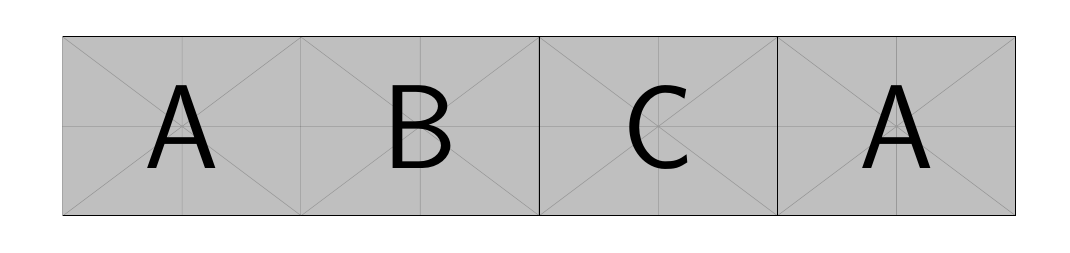
\begin{tikzpicture}
    \node[] (fig) at (0,0){
    \renewcommand{\arraystretch}{0}
    \begin{tabular}{c @{\hskip -0.2pt} c @{\hskip -0.2pt} c @{\hskip -0.2pt} c}
    \includegraphics[width=0.25\textwidth, origin=c]{example-image-a}&
    \includegraphics[width=0.25\textwidth, origin=c]{example-image-b}&
    \includegraphics[width=0.25\textwidth, origin=c]{example-image-c}&
    \includegraphics[width=0.25\textwidth, origin=c]{example-image-a}
    \end{tabular}};

\end{tikzpicture}
  \end{tabular}
  \end{tabular}}
\end{mdframed}
\end{document}